\documentclass[]{article}
\usepackage{lmodern}
\usepackage{amssymb,amsmath}
\usepackage{ifxetex,ifluatex}
\usepackage{fixltx2e} % provides \textsubscript
\ifnum 0\ifxetex 1\fi\ifluatex 1\fi=0 % if pdftex
  \usepackage[T1]{fontenc}
  \usepackage[utf8]{inputenc}
\else % if luatex or xelatex
  \ifxetex
    \usepackage{mathspec}
  \else
    \usepackage{fontspec}
  \fi
  \defaultfontfeatures{Ligatures=TeX,Scale=MatchLowercase}
\fi
% use upquote if available, for straight quotes in verbatim environments
\IfFileExists{upquote.sty}{\usepackage{upquote}}{}
% use microtype if available
\IfFileExists{microtype.sty}{%
\usepackage{microtype}
\UseMicrotypeSet[protrusion]{basicmath} % disable protrusion for tt fonts
}{}
\usepackage[margin=1in]{geometry}
\usepackage{hyperref}
\hypersetup{unicode=true,
            pdftitle={Introduction to Statistics for Data Science},
            pdfauthor={Katie Scranton, Senior Data Scientist, Precision Medicine},
            pdfborder={0 0 0},
            breaklinks=true}
\urlstyle{same}  % don't use monospace font for urls
\usepackage{graphicx,grffile}
\makeatletter
\def\maxwidth{\ifdim\Gin@nat@width>\linewidth\linewidth\else\Gin@nat@width\fi}
\def\maxheight{\ifdim\Gin@nat@height>\textheight\textheight\else\Gin@nat@height\fi}
\makeatother
% Scale images if necessary, so that they will not overflow the page
% margins by default, and it is still possible to overwrite the defaults
% using explicit options in \includegraphics[width, height, ...]{}
\setkeys{Gin}{width=\maxwidth,height=\maxheight,keepaspectratio}
\IfFileExists{parskip.sty}{%
\usepackage{parskip}
}{% else
\setlength{\parindent}{0pt}
\setlength{\parskip}{6pt plus 2pt minus 1pt}
}
\setlength{\emergencystretch}{3em}  % prevent overfull lines
\providecommand{\tightlist}{%
  \setlength{\itemsep}{0pt}\setlength{\parskip}{0pt}}
\setcounter{secnumdepth}{0}
% Redefines (sub)paragraphs to behave more like sections
\ifx\paragraph\undefined\else
\let\oldparagraph\paragraph
\renewcommand{\paragraph}[1]{\oldparagraph{#1}\mbox{}}
\fi
\ifx\subparagraph\undefined\else
\let\oldsubparagraph\subparagraph
\renewcommand{\subparagraph}[1]{\oldsubparagraph{#1}\mbox{}}
\fi

%%% Use protect on footnotes to avoid problems with footnotes in titles
\let\rmarkdownfootnote\footnote%
\def\footnote{\protect\rmarkdownfootnote}

%%% Change title format to be more compact
\usepackage{titling}

% Create subtitle command for use in maketitle
\newcommand{\subtitle}[1]{
  \posttitle{
    \begin{center}\large#1\end{center}
    }
}

\setlength{\droptitle}{-2em}

  \title{Introduction to Statistics for Data Science}
    \pretitle{\vspace{\droptitle}\centering\huge}
  \posttitle{\par}
    \author{Katie Scranton, Senior Data Scientist, Precision Medicine}
    \preauthor{\centering\large\emph}
  \postauthor{\par}
    \date{}
    \predate{}\postdate{}
  

\begin{document}
\maketitle

\subsection{Statistics is a way to identify patterns in the world that
we aren't able to see on our
own}\label{statistics-is-a-way-to-identify-patterns-in-the-world-that-we-arent-able-to-see-on-our-own}

We do this in the context of some question we are wondering about

\subsection{Example: Newborn birth
weight}\label{example-newborn-birth-weight}

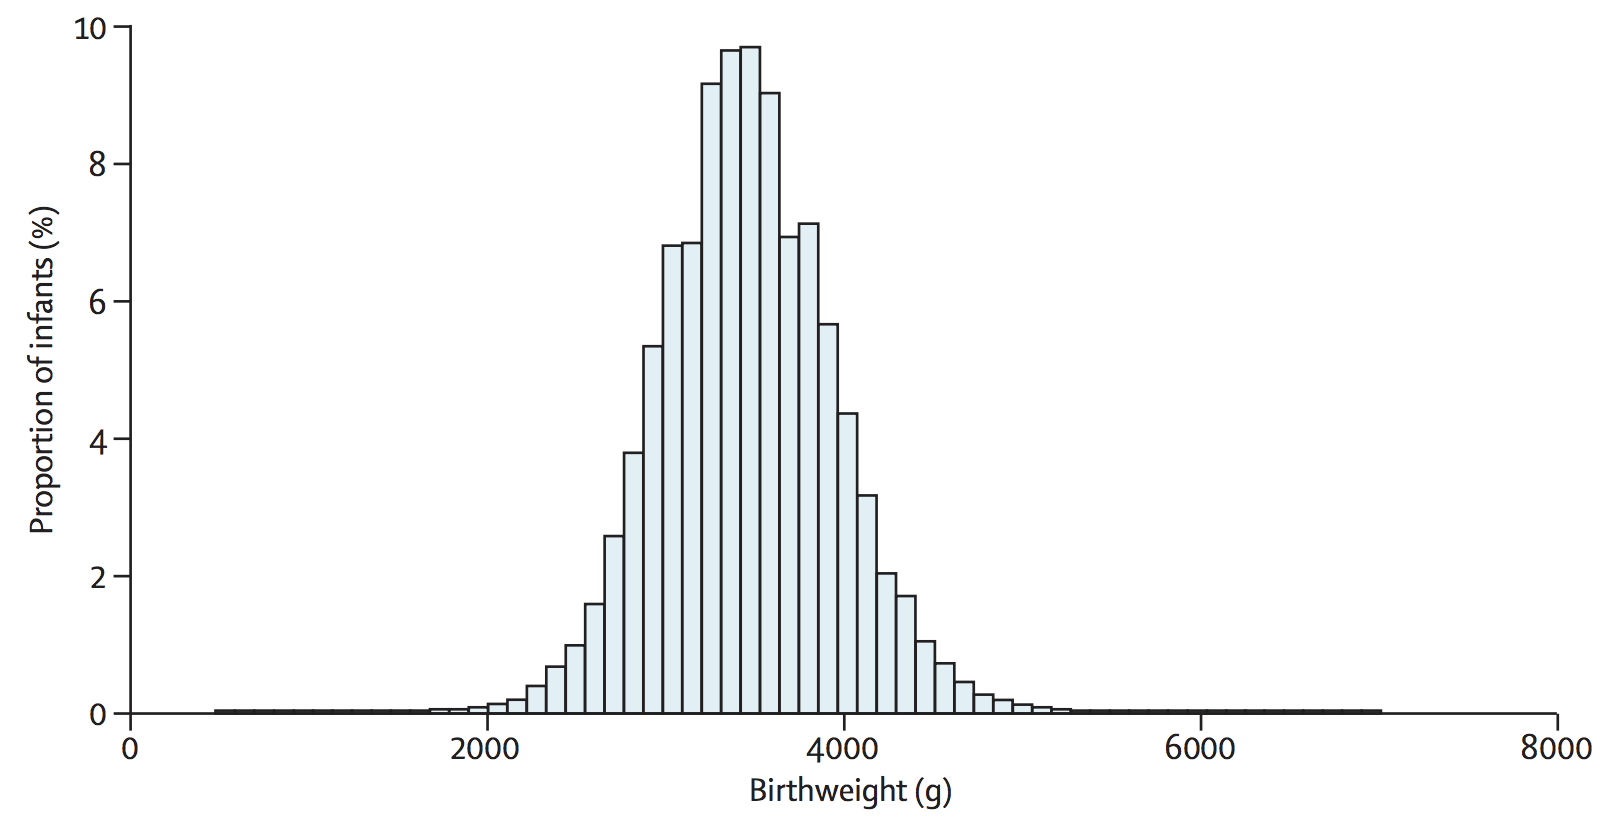
\includegraphics{images/lancet.png}
\href{https://www.thelancet.com/journals/lancet/article/PIIS0140-6736(10)60751-9/fulltext}{Ludwig
and Currie, 2010 The Lancet}

Let's say I'm a doctor at a hospital and I've noticed that in the past
month a few of my otherwise healthy patients have had very small babies.
I got suspicious and went back through their records. The only thing I
could find was that they were all taking a new brand of prenatal
vitamins. How can I gather evidence to decide whether the vitamins might
be the problem or its just a coincidence?

\includegraphics{IntroStats_files/figure-latex/hyptest-1.pdf}

\subsection{Hypothesis testing}\label{hypothesis-testing}

\begin{enumerate}
\def\labelenumi{\arabic{enumi}.}
\tightlist
\item
  I make a hypothesis:

  \begin{itemize}
  \tightlist
  \item
    Mothers taking this brand of vitamins have smaller babies
  \end{itemize}
\item
  I think of the the opposite hypothesis that would be kind of boring:

  \begin{itemize}
  \tightlist
  \item
    Mothers are just as likely to have small babies no matter what brand
    of vitamins they take
  \end{itemize}
\item
  I figure out what I can measure to \textbf{disprove} my null
  hypothesis

  \begin{itemize}
  \tightlist
  \item
    weight of each newborn
  \item
    average weight of all newborns whose mothers took the vitamins
  \item
    difference between the average weight of all newborns whose mothers
    took the vitamins and the average weight of all newborns whose
    mothers took other vitamins
  \end{itemize}
\item
  If I could repeat this experiment many many times and the null
  hypothesis is always true, what kind of results would I get?
\end{enumerate}

Well if there is no real effect of the vitamins then the differences
between the two groups will usually be zero. But just by chance maybe
one group of babies has a few very large newborns or a few smaller
newborns. So there will be random differences between any two groups you
pick.

We know the differences between two groups (that are really from the
same large population) will usually be zero (mean = 0) and there will be
some variation due to random chance. We could expect that variation will
get smaller if we take larger samples so any one large baby has less of
an effect on the average.

\paragraph{This is called a null
distribution!}\label{this-is-called-a-null-distribution}

The distribution of whatever you are measuring under the null hypothesis

In this case, if the mean is zero and the variation gets smaller with
larger sample size, then the distribution is a t distribution, similar
to a Normal distribution.

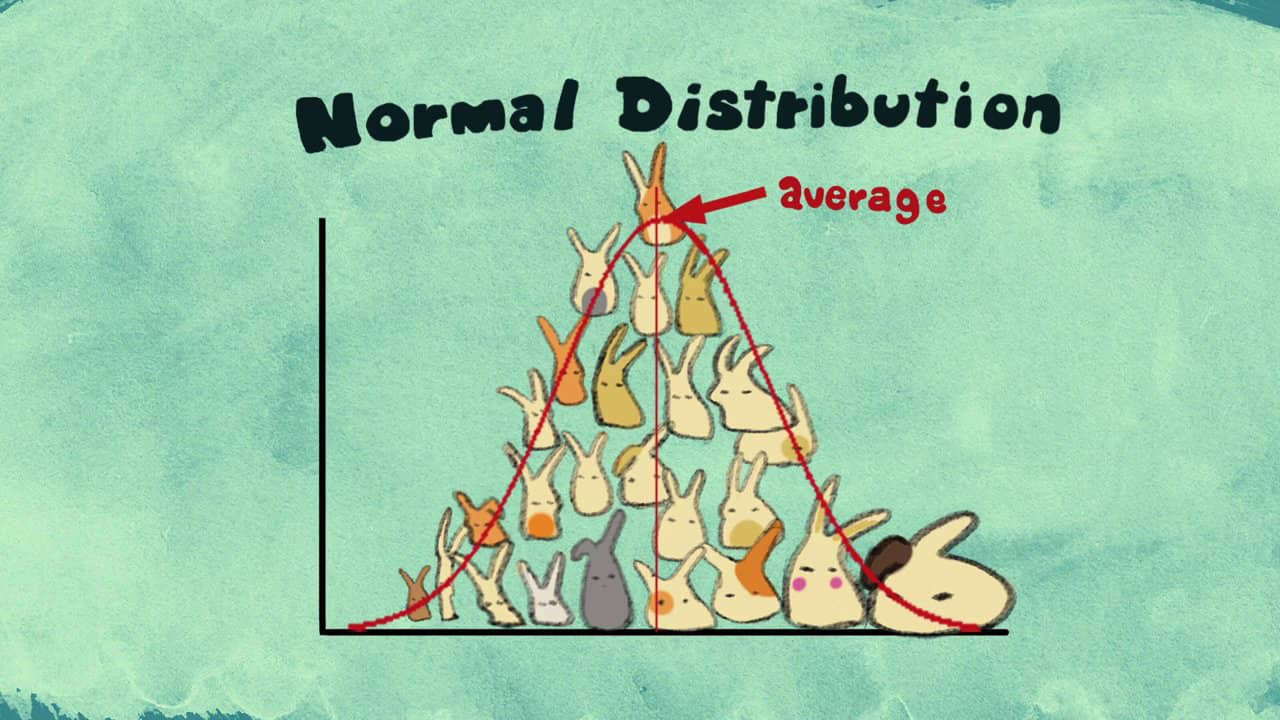
\includegraphics{images/distributions.jpeg}
\href{https://vimeo.com/75089338}{source}

\includegraphics{IntroStats_files/figure-latex/birthweighthist-1.pdf}

\subsubsection{\texorpdfstring{About
\(\color{cyan}{\text{68% of the area}}\) includes the mean plus or minus
1 standard
deviation}{About \textbackslash{}color\{cyan\}\{\textbackslash{}text\{68\% of the area\}\} includes the mean plus or minus 1 standard deviation}}\label{about-colorcyantext68-of-the-area-includes-the-mean-plus-or-minus-1-standard-deviation}

\subsubsection{\texorpdfstring{About
\(\color{orange}{\text{95% of the area}}\) includes the mean plus or
minus 2 standard
deviation}{About \textbackslash{}color\{orange\}\{\textbackslash{}text\{95\% of the area\}\} includes the mean plus or minus 2 standard deviation}}\label{about-colororangetext95-of-the-area-includes-the-mean-plus-or-minus-2-standard-deviation}

Back to the newborns \ldots{}

\includegraphics{IntroStats_files/figure-latex/ttest1-1.pdf}

We're measuring the differences between the averages of each group. If
the null hypothesis were true, and we repeat this experiment over and
over again, the difference between two groups will usually be zero, but
sometimes just due to chance one sample will have larger babies than the
other.

\includegraphics{IntroStats_files/figure-latex/ttest2-1.pdf}

We can compare the actual difference we noticed in the hospital to the
\textbf{null distribution} to ask:

\paragraph{What is the probability that the differences we see in real
life are due to random chance not the
vitamins?}\label{what-is-the-probability-that-the-differences-we-see-in-real-life-are-due-to-random-chance-not-the-vitamins}

\includegraphics{IntroStats_files/figure-latex/ttest3-1.pdf}

\paragraph{\texorpdfstring{The
\(\color{green}{\text{green area of the curve}}\) is
\ldots{}}{The \textbackslash{}color\{green\}\{\textbackslash{}text\{green area of the curve\}\} is \ldots{}}}\label{the-colorgreentextgreen-area-of-the-curve-is}

\paragraph{the probability that a random sample of babies would have a
lower average birthweight than our vitamin
babies}\label{the-probability-that-a-random-sample-of-babies-would-have-a-lower-average-birthweight-than-our-vitamin-babies}

\subsubsection{The chance of seeing a group of random babies who weighed
less on average than our group is
0.3123\%.}\label{the-chance-of-seeing-a-group-of-random-babies-who-weighed-less-on-average-than-our-group-is-0.3123.}

This value is our p-value: the probabilty that random chance could
produce data as, or more, extreme than the observed data

Usually we use a cutoff of 5\% for p-values: We say the data are not
just a coincidence, or vitamin brand has a significant effect, if the
probabilty that random chance could produce data as, or more, extreme
than the observed data, is less than 5\%.

\paragraph{But significance levels (p=0.05) are
arbitrary!!!}\label{but-significance-levels-p0.05-are-arbitrary}

\subsection{Hypothesis testing is the same for every
test!!}\label{hypothesis-testing-is-the-same-for-every-test}

\paragraph{1. For any question, what is your
hypothesis?}\label{for-any-question-what-is-your-hypothesis}

\paragraph{2. For any hypothesis, what would be the
alternative?}\label{for-any-hypothesis-what-would-be-the-alternative}

\paragraph{3. For any hypothesis, what statistic could you measure to
evaluate
it?}\label{for-any-hypothesis-what-statistic-could-you-measure-to-evaluate-it}

\paragraph{4. If you repeated this experiment many many times and the
alternative were true, what would the histogram of statistics you
measure look
like?}\label{if-you-repeated-this-experiment-many-many-times-and-the-alternative-were-true-what-would-the-histogram-of-statistics-you-measure-look-like}

\paragraph{5. Ask how likely it is that random chance could produce data
as, or more, extreme than the observed
data}\label{ask-how-likely-it-is-that-random-chance-could-produce-data-as-or-more-extreme-than-the-observed-data}

\section{Errors}\label{errors}

\includegraphics{IntroStats_files/figure-latex/errors-1.pdf}

\paragraph{\texorpdfstring{The
\(\color{red}{\text{red area of the curve}}\) are the groups of babies
that just by chance hapen to have lowest average birth weight, compared
to the rest of the
population.}{The \textbackslash{}color\{red\}\{\textbackslash{}text\{red area of the curve\}\} are the groups of babies that just by chance hapen to have lowest average birth weight, compared to the rest of the population.}}\label{the-colorredtextred-area-of-the-curve-are-the-groups-of-babies-that-just-by-chance-hapen-to-have-lowest-average-birth-weight-compared-to-the-rest-of-the-population.}

If the newborns in your experiment just happened to be one of these
groups you would mistakenly conclude that the vitamins may have an
adverse effect, even though there is no difference. This would be a
false positive. By setting our significance level to 0.05 we know that
5\% of the time we conduct an experiment we will make this error.

We could also make the opposite error: concluding that the vitamins are
not associated with low birth weights, even though they are. To know how
often we would make that mistake we would have to have some knowledge of
the larger distribution of birth weights for mothers who took those
vitamins.

 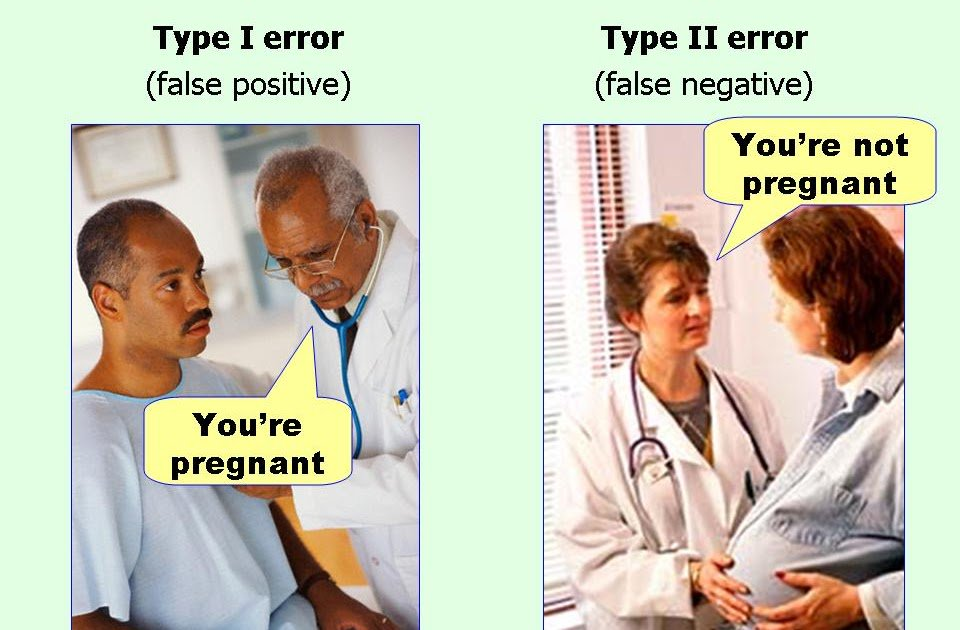
\includegraphics{images/errors-I-II.jpeg}
\href{https://twitter.com/phiktn}{photo credit}

\includegraphics{IntroStats_files/figure-latex/birthweightgender-1.pdf}

\includegraphics{IntroStats_files/figure-latex/auc1-1.pdf}

\includegraphics{IntroStats_files/figure-latex/auc2-1.pdf}

\subsection{Confidence Intervals}\label{confidence-intervals}

\includegraphics{IntroStats_files/figure-latex/confint1-1.pdf}

\paragraph{What if we just want to estimate the average weight of a
newborn?}\label{what-if-we-just-want-to-estimate-the-average-weight-of-a-newborn}

Easy! It is 3289.45g.

But we know that this mean is calculated using only the babies born in
that hospital over a certain period of time. If you repeated the
experiment in a different hospital or over a different time period you
might get a slightly different answer to to random chance alone. So it
is important to estimate the error around a mean (or any other
statistic).

So lets think about what the null distribution of means would look like.
If you estimates the mean birth weight over and over, you end up with a
distirbution of means with some variation where occasionally you get a
group of babies that are on average slightly overweight or slightly
underweight.

\includegraphics{IntroStats_files/figure-latex/confint2-1.pdf}

We know that variation goes down with sample size. So we use our
\textbf{null distribution} to find the range that will give us the
\(\color{orange}{\text{95%}}\) range. For a Normal distribution this is
the mean plus or minus \emph{about} 2 standard deviations.

Once we sample a group of babies and estimate the average, we estimate
the standard error and calculate the confidence interval.

\subsubsection{\texorpdfstring{This \(\color{orange}{\text{95%}}\)
confidence interval (CI) represents a range, that if you did this
experiment over and over, calculated the CI over and over, 95\% of the
time it would overlap the true population mean birth
weight.}{This \textbackslash{}color\{orange\}\{\textbackslash{}text\{95\%\}\} confidence interval (CI) represents a range, that if you did this experiment over and over, calculated the CI over and over, 95\% of the time it would overlap the true population mean birth weight.}}\label{this-colororangetext95-confidence-interval-ci-represents-a-range-that-if-you-did-this-experiment-over-and-over-calculated-the-ci-over-and-over-95-of-the-time-it-would-overlap-the-true-population-mean-birth-weight.}

\begin{figure}
\centering

\includegraphics{images/intro.png}
\caption{}
\end{figure}

\begin{figure}
\centering
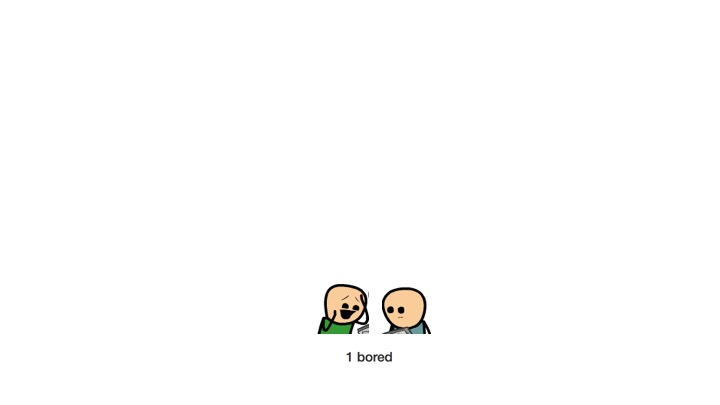
\includegraphics{images/Slide1.jpeg}
\caption{}
\end{figure}

\begin{figure}
\centering
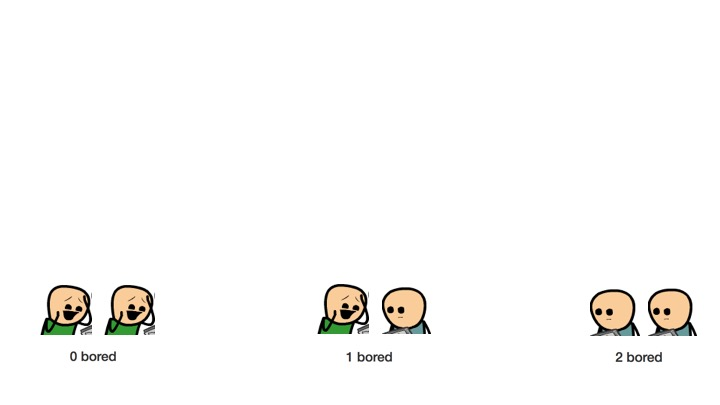
\includegraphics{images/Slide2.jpeg}
\caption{}
\end{figure}

\begin{figure}
\centering
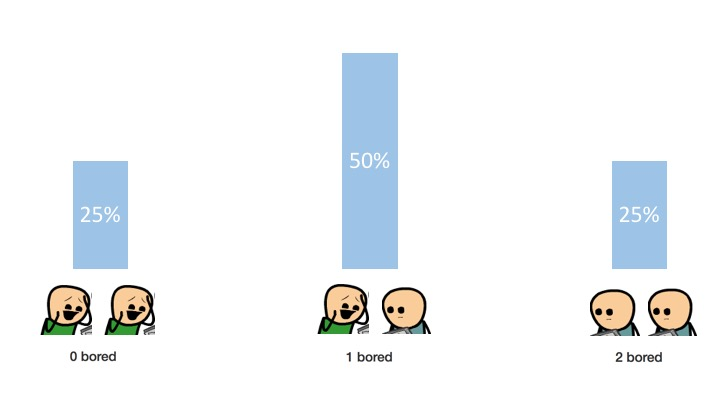
\includegraphics{images/Slide3.jpeg}
\caption{}
\end{figure}

\subsection{Binomial distribution}\label{binomial-distribution}

\begin{itemize}
\item
  Binary - either yes or no, heads or tails, bored or not
\item
  Coin flip - 50\% chance each person here is bored by statistics
\item
  Weighted coin - unfair - not necessarily 50\%
\item
  For a repeated number of coin flips, how many are heads?
\end{itemize}

\subsection{Example: Newborn gender}\label{example-newborn-gender}

\includegraphics{IntroStats_files/figure-latex/gender-1.pdf}

\subsection{Linear regression}\label{linear-regression}

\includegraphics{IntroStats_files/figure-latex/birthweight-1.pdf}

We'd like to draw a line on the graph that is the best approximation to
the data.

\includegraphics{IntroStats_files/figure-latex/bwreg1-1.pdf}

\includegraphics{IntroStats_files/figure-latex/bwreg2-1.pdf}

\includegraphics{IntroStats_files/figure-latex/bwreg3-1.pdf}

\subsection{Logistic regression}\label{logistic-regression}

\section{Bayesian analysis}\label{bayesian-analysis}

Frequentists would say:

I could do an experiment of picking up random items and measuring the
distance to the ocean and calculate the average distance to the ocean
and repeat that experiment many many times. If its true that seashells
are just as likely to be found near the ocean as any random item, then

The proportion of times I did that experiment with something other than
a seashell and ended up closer to the ocean than I did with the seashell
is the probability I'm near the ocean, given that I picked up a
seashell.

Bayesian statistics don't live in a universe where you need to think of
hypothetically repeating experiments many many times.

\begin{figure}
\centering
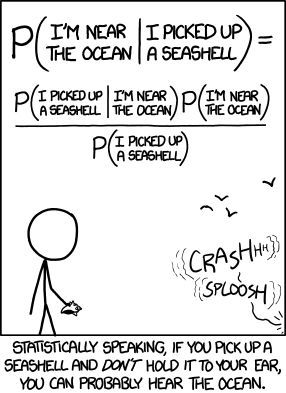
\includegraphics{images/content_bayes.jpg}
\caption{}
\end{figure}

\href{https://twitter.com/seanjtaylor/status/1073632404286275584}{source}


\end{document}
